\documentclass[11pt]{article}

\usepackage[english]{babel}
\usepackage[utf8]{inputenc}
\usepackage{amsmath}
\usepackage{amssymb}
\usepackage{setspace}
\usepackage{graphicx}
\usepackage{apacite}
\usepackage{caption}
\usepackage{subcaption}

% \usepackage[
% backend=biber,
% style=alphabetic,
% citestyle=apa
% ]{biblatex}

% \addbibresource{references.bib} % imports bibliography file
\graphicspath{ {./images/}} % Import images 

\title{% 
    Validate Structural Analysis \\ 
    \large Testing GPV Method in First-Price Reverse Auctions}

\author{Qingbo Liu\\[0.5cm]{\small Advisor: Timothy P. Hubbard}}

% \doublespacing
\onehalfspacing
\begin{document}
\maketitle

\section{Introduction}
% previous version  
% Auctions are a price-discovering mechanism in environments where there is no 
% well established known price for items. Participants at auctions have heterogenous
% valuations about the items being auctioned. The standard economic assumption is that 
% bidders draw independent or affalidated valuations before the auction starts and 
% submit their bids as a possibly 
% non-linear function of their valuations and preferences. At the end, winners 
% are determined according to certain rules. At the momement the winner is designated, 
% a particular objective of the auction mechanism that is employed is achieved, 
% such as social welfare maximization, revenue maximiaztion, etc. 

% However, there are certain cases where the theory is unlikely to match the reality. 
% For example, in first-price auctions, the usual economic model on bidders' 
% behavior draws on an important concept -- equilibrium. The notion of equilibrium 
% states that if every participant in the auction adopts the equilibrium strategy, 
% no one can gain more advantage by switching to a modified strategy and the 
% equilibrium is achieved usually through repeated playing. The theory 
% predicts that in first-price sealed-bid auctions bidders would bid a 
% fractional part of their values, dependent on the number of participants. 
% The intuition behind the theory is that the larger the number of bidders 
% in a given auction, the more fierce the competition is.  
% The theory is elegant, but the complexities inherent in real life are 
% likely to render the model less predictive than it should suggest. 

% The fact that theoretical models might not give reliable predictions 
% has implications for works that rely on them. Structural analysis, 
% which uses statistical tools to infer models's parameters from data and 
% gives predictions based on the data, is especially vulnerable to this attack. 
% For instance, the predicted bidding behavior in first-price sealed-bid auctions 
% might not hold in reality, as demonstrated by the lab study Neugebauer \& Selten (2004). 
% Yet Harrison (1989) also raises methodological critique of the lab experiments 
% in the way of comparison. [more details on this]

% But lab experiment is ultimately different from real auctions and it remains an open 
% problem to empirically verify the effectiveness of theoretical predictions, which 
% is the goal of this paper. This paper tries to address the question of 


% what structural analysis enables us to do, its drawbacks and the introduction 
% of machine learning practices to verify the if it is correct

Participants at auctions submit bids for items based on their valuations and 
preferences of the items. There are many ways to think about the transformation from 
valuations and preferences into bids, and the usual economic approach is to consider 
the bids as a mathematical function of valuations and preferences, an approach which 
this paper will take. At the end of auctions, the winner(s) 
is designated based on certain auction rules and the auction data becomes available.
The data includes only bids, the final output of the bidding function, and the inputs, 
valuations and preferences, remain unknown. Yet interesting and useful analysis 
of auctions entails the knowledge about valuations and preferences. For example, 
to evaluate the performance of auctions, it is necessary to have access to bidder's 
valuations to determine if the particular mechanism has achieved its objective,
which leads to structural estimation. 

Structural estimation assumes a particular model and uses statistical methods to 
estimate relevant parameters of the model. The calibrated model can then 
give predictions regarding objects that are being investigated. For example, 
in first-price sealed-bid reverse auctions, 
one of the mechanisms that the government uses for public project procurements, 
the simple assumption is that all participants independently draw costs from an 
identical cost distribution. 
Each bidder submits a sealed bid to the auctioneer and after all bidders have finished 
submission the winner is the one with the lowest bid. With this bidding model, 
structural estimation can be used 
to infer the cost distribution based on observed bids \cite{Guerreetal2000}.
Compared to regression analysis, structural estimation imposes a stringer set of 
assumptions on the data. But more than just discovering the correlation between 
variables as regression analysis does, structural estimation is able to produce stronger 
counter-factual predictions, such as the cost distribution as mentioned above. 

The central assumption underlying structural estimation is that the model used 
is correct in a particular environment. To overcome such a drawback, alternative 
studies such as lab experiments are used to confirm the theory's validity. But 
laboratory environments ultimately differ from the real environments and 
the conclusions from laboratory studies may not hold in more realistic environments. 
The goal of this paper is to test model validity in a new different way by 
borrowing the techniques from statistical learning literature. In statistical 
learning, multiple models for predictive purposes are trained on part of the dataset 
and their performance is evaluated on another reserved split of 
the available dataset. The technique is called cross-validation 
and is used when there are candidate models and their performance needs to 
be compared to select the fittest one. In this paper, I will adapt the idea 
of cross-validation to test the predictiveness of economic models. By splitting 
data into training data and test data as in statistical learning, I will 
run structural estimation on the training data, simulate test data using the 
results from structural estimation, and compare the simulated data to actual 
test data. If the difference is statistically significant, that suggests 
unfitness of the model in the particular environment. 
In this paper, I will use data from government procurement auctions to test 
the first-price sealed-bid equilibrium model \cite{RileySamuelson1981} 
for structural estimation
\footnote{The original goal of this paper also includes comparing the cost 
distribution of DBE/MBE/WBE (standing respectively for Disadvantaged/Minority/Woman
Business Enterprise) to the cost distribution of other firms, which will add 
to the existing literature on understanding how DBE/MBE/WBE perform relative 
to other firms. But due to data availability on these types of firms 
and time constraints on the project as this is a 
term paper, this goal is omitted. }.

Similar work has been done in \citeauthor{ChernomazYushioto2019} 
\citeyear{ChernomazYushioto2019}, where they have compared the accuracy 
of semiparametric and nonparametric structural estimation methods in an 
asymmetric environment.  

The remainder of the paper is organized as follows. Section 2 discusses the 
characteristics of the environment and derives the model for structural 
estimation. Section 3 examines the data and presents estimation results. 
Section 4 runs simulations based on estimation. Section 5 concludes with 
a discussion on the results and possible improvements. 

\section{Model}

For the model setup, suppose there are $n$ bidders in the auction, with 
$n \geq 2$, and 
there is a single, indivisible object being auctioned. Each bidder submits 
a sealed bid based on an observed cost before the auction. The 
bidder's cost $c$ is drawn i.i.d from a common distribution $F(\cdot)$ which is 
continuous with density $f(\cdot)$ on the support $[\underline{c}, \overline{c}] \subset \mathbb{R}^{+}$. 
All bidders are quasi-linear utility-maximizers, with the utility function 
$u(c, b) = b - c$. Bidders are therefore assumed to be risk-neutral. 
The number of bidders $n$, the cost distribution $F$ and its support are common 
knowledge to all bidders in the auction. Besides, each bidder $i$ can only observe her 
private cost $c_i$ and no one else's. 

Different from first-price sealed-bid auctions where 
the highest bidder wins, in first-price sealed-bid reverse 
auctions the winner is the one who submits the 
lowest bid. In the following subsection, I will derive the 
Bayes-Nash Equilibrium in the FPSB reverse auction environment.
After I have characterized the equilibrium, now I will proceed to describe how 
private costs can be inferred from observed bids based on the equilibrium. 

\subsection{Bayes-Nash Equilibrium}
For bidder $i$ in the auction, she needs to report a bid $b_i$ based on 
her private cost $c_i$. The bidder achieves maximal utility 
by maximizing the function 
$$ \max_{b_i} (b_i - c_i)P(\text{win}|b_i), $$ 
which is saying by picking an appropriate bid $b_i$, the bidder 
has a good balance between the revenue and probability of winning. 

Since this is a first-price reverse auction, where the lowest bidder wins, 
the probability of winning is 
\begin{align*}
    P(\text{win}|b_i) &= P(b_1 \geq b_i, ... b_{i-1} \geq b_i, b_{i+1} \geq b_i, ... b_n \geq b_i) \\
        &= P(b_1 \geq b_i) ... P(b_{i-1} \geq b_i) P(b_{i+1} \geq b_i) ... P(b_n \geq b_i) \\
        &= [1-P(b_1 \leq b_i)] ... [1-P(b_{i-1} \leq b_i)][1-P(b_{i+1} \leq b_i)] ... [1-P(b_n \leq b_i)] \\
        &= \prod_{j=1, j \neq i}^{N}[1-P(b_j \leq b_i)]
\end{align*}

Now, suppose that there is a monotone bidding equilibrium function $s(\cdot)$ such that 
all bidders abide by it and makes their bids based on it, i.e. $b_i = s(c_i)$. 
Then
\begin{align*}
    P(\text{win}|b_i) &= \prod_{j=1, j \neq i}^{N}[1-P(s(c_j) \leq b_i)] \\ 
        &= \prod_{j=1, j \neq i}^{N}[1-P(c_j \leq s^{-1}(b_i))] \\ 
        &= \prod_{j=1, j \neq i}^{N}[1-F(s^{-1}(b_i))] \\ 
        &= [1-F(s^{-1}(b_i))]^{n-1}, 
\end{align*}
where the last equality follows from symmetry -- all bidders draw costs (independently) 
from the same distribution. 

The objective function therefore becomes 
$$ \max_{b_i} (b_i - c_i)[1-F(s^{-1}(b_i))]^{n-1}$$ 
and setting the derivative of it with respect to $b_i$ equal to 0 yields
\begin{align}
    [1-F(s^{-1}(b_i))]^{n-1} &= (b_i -c_i)(n-1)[1-F(s^{-1}(b_i))]^{n-2}f(s^{-1}(b_i))\frac{d s^{-1}(b_i)}{d b_i} \nonumber \\
    [1-F(c_i)]^{n-1} &= (s(c_i) -c_i)(n-1)[1-F(c_i)]^{n-2}f(c_i)\frac{1}{s'(c_i)} \nonumber \\
    1 &= (s(c_i)-v_i)(n-1)\frac{f(c_i)}{1-F(c_i)}\frac{1}{s'(c_i)}     \label{eqn:BiddingDiffQ}
\end{align}

The differential equation characterizes the strategy in sealed-bid first-price 
reverse auction and the solution of it, $s(\cdot)$, gives the equilibrium 
bidding function as follows \cite{HubbardPaarsch2009}
\begin{equation}
    s(c) = b =  c + \frac{\int_c^{\overline{c}} [1 - F(u)]^{n-1} du}{[1 - F(c)]^{n-1}}
    \label{eqn:BiddingFunction}
\end{equation}


\subsection{Cost Inference}
Our interest, however, lies not in the particular solution 
of this differential equation, but in using it as an intermediate step 
in deriving cost as a function of bids, i.e. $s^{-1}(\cdot)$.

Assume $G(\cdot)$ represents the cumulative distribution of bids, 
along with the continuous density function $g(\cdot)$ and support 
$[\underline{b}, \overline{b}] = [s(\underline{c}), s(\overline{c})]$.
As in \citeauthor{Guerreetal2000} \citeyear{Guerreetal2000}, by a transformation of random variables, I have the identity 
$G(b) = P(\tilde{b} < b) = P(\tilde{c} < s^{-1}(b)) = F(s^{-1}(b)) = F(c)$
and $g(b) = f(c) /s'(c)$. The ratio of $g(b)/(1 - G(b))$ gives 
$f(c_i)/(1-F(c_i))(1/s'(c_i))$. From this, equation (\ref{eqn:BiddingDiffQ}) becomes 
\begin{equation}
    \label{eqn:ReverseFunction}
    c_i = b_i - \frac{1}{n-1}\frac{g(b_i)}{1-G(b_i)}
\end{equation}

In an environment of $n$ bidders, Equation (\ref{eqn:ReverseFunction}) provides 
the method to estimate pseudo-costs from observed bids with kernel-estimated 
bid density and bid distribution. The estimated costs are pseudo because of  
assumptions that bidders are risk-neutral and play a Bayes-Nash equilibrium bidding 
strategy. 

\subsection{Estimation}
The estimation consists of two steps. In step 1, I recover costs $c$ based on 
observed bids $b$, by first non-parametrically estimating $G(b)$ and $g(b)$ 
and then using equation (\ref{eqn:ReverseFunction}) to 
generate pseudo-costs. In the second step, I can non-parametrically estimate the cost
density $f(c)$ from pseudo-costs. 

The technique used to estimate $G(b)$ and $g(b)$, as well as $f(c)$, is called 
kernel density estimation and has the following form
\begin{equation}
    \hat{f}(x) = \frac{1}{nh}\sum_{i=1}^n K(\frac{x-x_i}{h}),
    \label{eqn:KDE_f}
\end{equation}
and 
\begin{equation}
    \hat{F}(x) = \frac{1}{n}\sum_{i=1}^n I(x_i \leq x), 
    \label{eqn:KDE_F}
\end{equation}
where I have a set of observables ${x_1, x_2, ... x_n}$. However, this  
kernel density estimation (\ref{eqn:KDE_f}) 
method suffers from boundary 
problem and instead, I will use the boundary-corrected kernel estimation 
method as proposed in \cite{HickmanHubbard2015}

This two-step estimation method has the advantage that to estimate cost 
distribution with observed bids, I do not need to assume a prior distribution 
of $f(c)$ to estimate it (which is a parametric method that works by 
first assuming the shape of a distribution and then estimating parameters of the 
distribution from data). 


\section{Data and Results}
The bidding data used in this paper is downloaded from the Colorado Department of 
Transportation (https://www.codot.gov/business/bidding). I will take a short detour of the data itself before 
presenting results on cost estimation. 

\subsection{Data Description}
\begin{table}[h!]
    \centering
    \begin{tabular}{|l|l|l|l|l|l|}
    \hline
                                       & Mean         & Median       & \begin{tabular}[c]{@{}l@{}}Standard\\ Deviation\end{tabular} & Max           & Min  \\ \hline
        Total Bid                      & 3,172,164.68 & 1,366,571.20 & 5,491,805.02                                                 & 93,398,000.00 & 0.00 \\ \hline
        \begin{tabular}[c]{@{}l@{}}Percent of Engineer's\\ Estimate (Cost)\end{tabular} & 106.54       & 100.02       & 22.63                                                        & 750.00        & 0.00 \\ \hline
        Number of Bidders              & 5.47         & 5            & 2.5                                                          & 16            & 1    \\ \hline
\end{tabular}
\caption{Basic summary statistics of data}
\label{table:1}
\end{table}

There are in total 1182 auctions in the data. For each auction, I have 
the number of participants $n$, bids submitted by participants and the engineer's 
estimate. The summary statistics of the data are summarized in Table \ref{table:1}. 
Projects vary from each other in their sizes, types, and many other factors. 
Even the same type of projects will have different costs. As Table \ref{table:1}
shows, the variance in Total Bid is very large and not an ideal candidate for 
cost estimates. Instead, I will work with Percent of Engineer's Estimate to 
infer cost distribution. Percent of Engineer's Estimate is Total Bid divided 
by Engineer's Estimate, which is also known as normalized bids. 
Inferred cost distribution constructed this way will be invariant 
across projects. 

\begin{figure}
    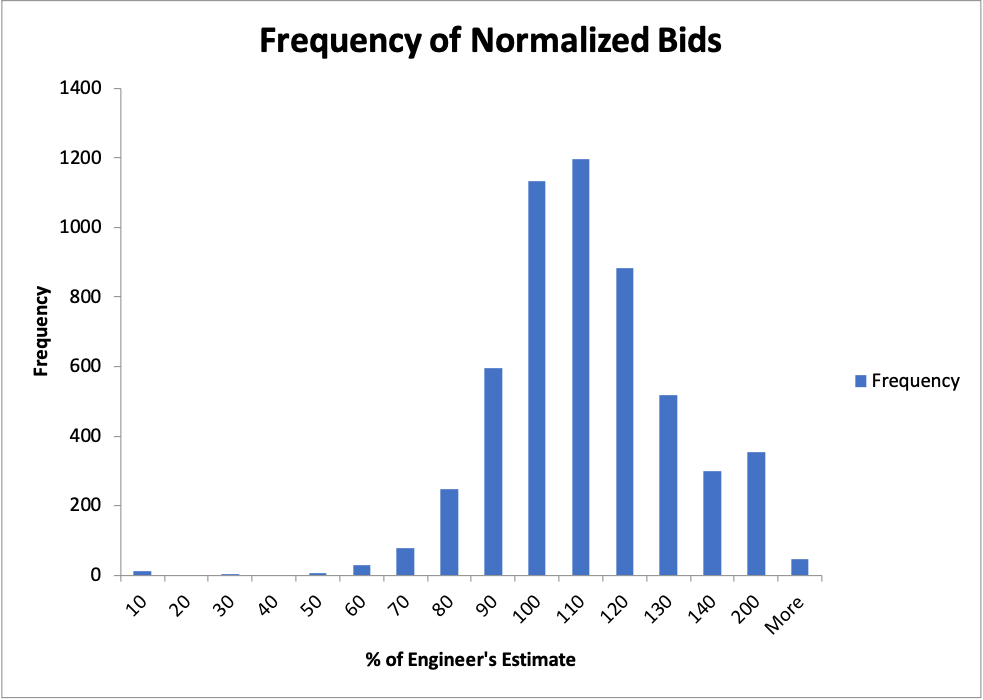
\includegraphics[width=0.8\textwidth]{BidFrequency.png}
    \centering
    \caption{Frequency of normalized bids (bids divided by engineer's estimate)}
    \label{fig:BidFrequency}
\end{figure}

Figure \ref{fig:BidFrequency} plots the frequency of normalized bids. Most bids 
are centered around $110\%$, which is slightly higher than the engineer's estimate 
with respect to which bids are normalized.
However, there are some outliers located in the \textit{More} bin, 
which would cause numeric instability in estimation. 
For data that is More bins, the kernel-estimated bid distribution 
$G_B(\cdot)$ is close to $1$ and so $1-G_B(\cdot)$ close to 0. As in 
the right-hand side of equation (\ref{eqn:ReverseFunction}), the 
part $\frac{g(b)}{1-G_B{b}}$ will tend to infinity as $1-G_B(b)$ 
approaches zero, resulting in the estimated cost to be negative. 
The problem will persist over the boundary of the data and is 
inherent in the kernel distribution estimation.
The boundary-correction technique introduced in \cite{HickmanHubbard2015}
applies only to the kernel density estimation, not kernel 
distribution estimation, and overcoming 
the boundary problems in kernel distribution estimation is outside the scope 
of this paper. For simplicity, I will first use equation 
(\ref{eqn:ReverseFunction}) to estimate costs and then trim the negative costs.

\subsection{Results}
With data comprised of auctions that have a different number of participants, 
the general estimation procedure remains the same. But the equation 
(\ref{eqn:ReverseFunction}) that assumes a fixed $n$ for the number 
of participants is modified to 
accommodate varying $n$ \cite{Matthewetal2018}
\begin{equation}
    c_{in} = b_{in} - \frac{1}{n-1} \cdot \frac{g(b_{in}|N = n)}{1-G_{B}(b_{in}|N=n)},
    \label{eqn:ReverseFunction_N}
\end{equation}
where $c_{in}$ and $b_{in}$ refer to the cost and bid in $i$-th auction 
with $n$ participants, and the density $g(\cdot|N=n)$ and distribution
$G(\cdot|N=n)$ are estimated on auction data with $n$ participants. 

\begin{figure}
    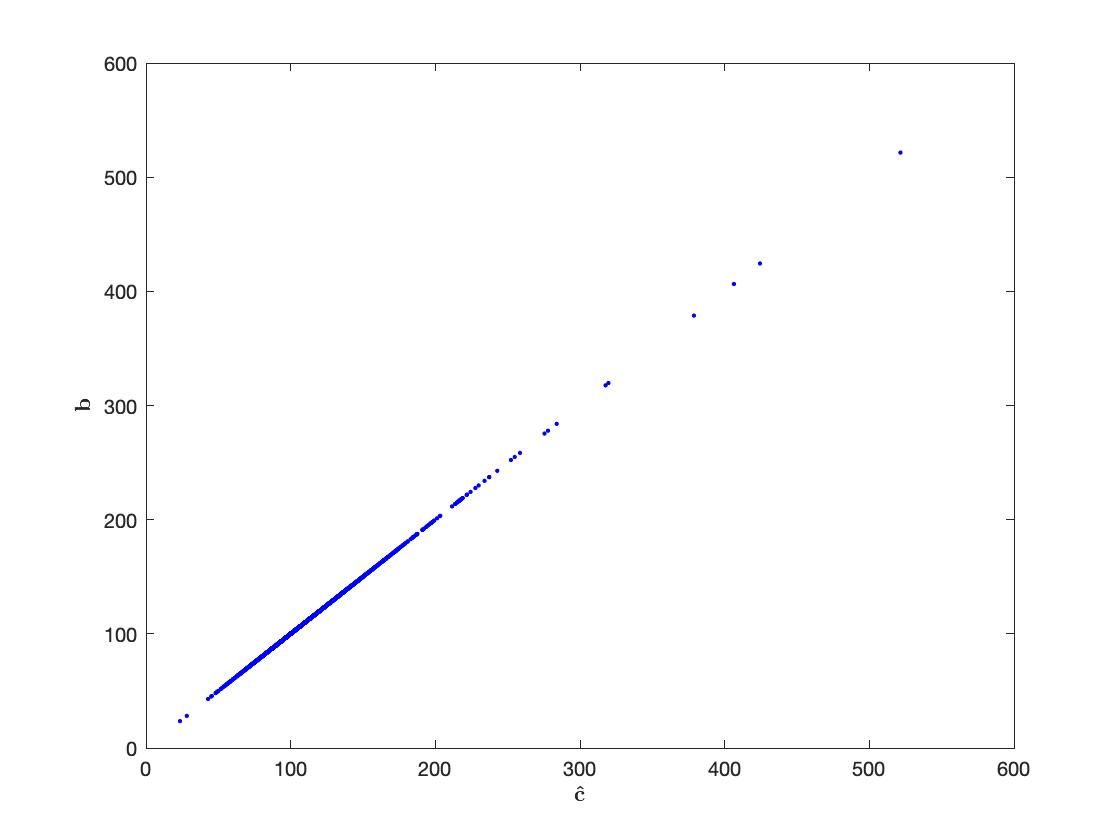
\includegraphics[width=0.75\textwidth]{cost_bid.jpg}
    \centering
    \caption{Estimated costs plotted against bids.}
    \label{fig:cost_bid}
\end{figure}

Figure \ref{fig:cost_bid} plots the estimated cost against bids in the plot. 
Bidder's markup over costs is infinitesimal. This is so 
mainly due to the bid distribution. As shown in Figure \ref{fig:BidFrequency}, 
most of the bids are scattered in the range [70, 200], which means that for each 
bid $b$, the estimated density value at the specific bid value, $f_c(b)$, is 
small: the peak of $f_c(\cdot)$ being $0.0222$. A closer look at the bid 
distributions of auctions with a different number of participants, $n$, reveals 
that the majority of auction data with small $n$, where the competition is less 
fierce and bidders are able to have a larger markup over the costs than those 
having more competitors, has bids compressed around $110\%$. The fact 
that bids and costs are very close also suggests that the auctions are 
very efficient in helping the Colorado government save money. 

\begin{figure}
\centering
    \begin{minipage}[h]{0.5\textwidth}
        \centering
        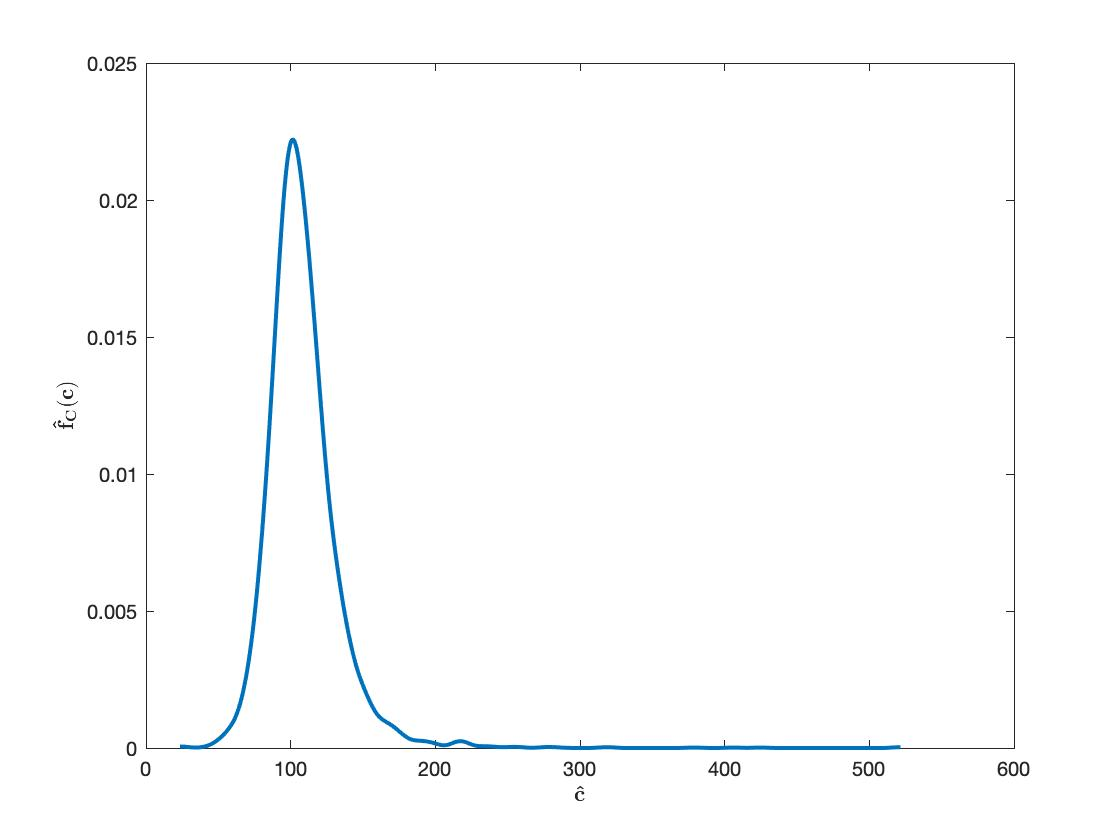
\includegraphics[width=1\linewidth]{costDensity.jpg}
    \end{minipage}%
    \begin{minipage}[h]{0.5\textwidth}
        \centering
        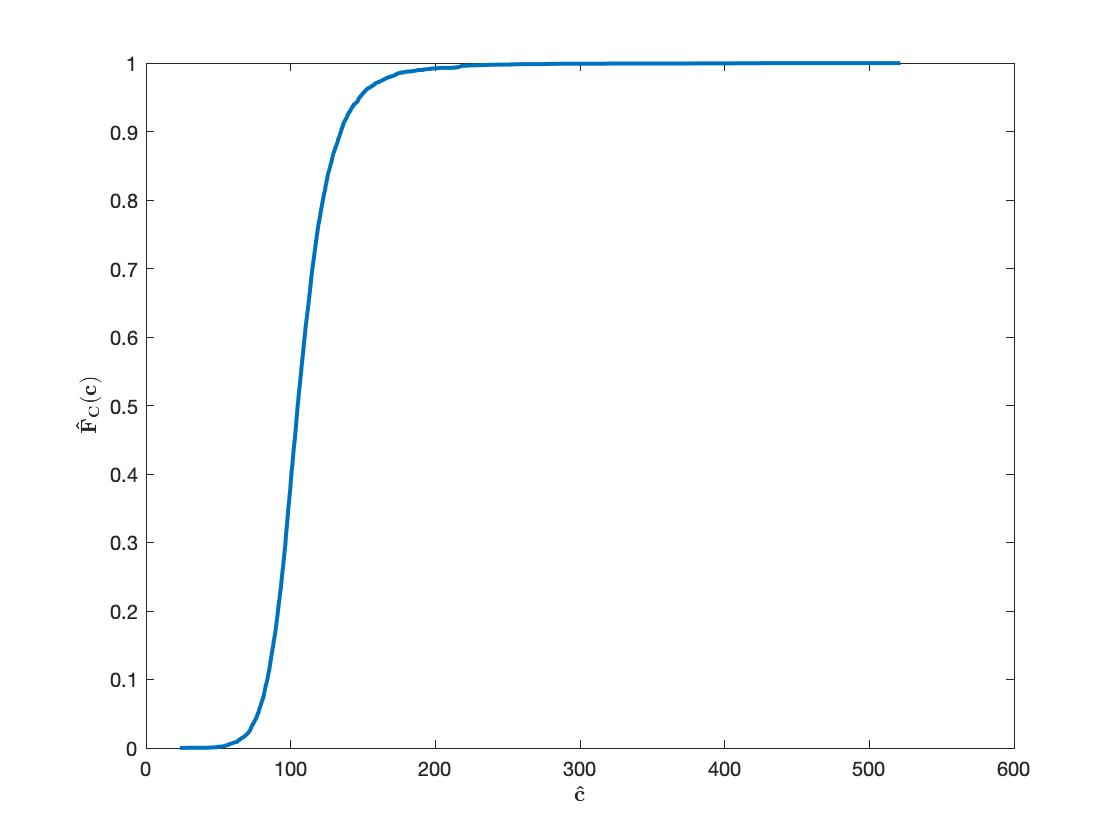
\includegraphics[width=1\linewidth]{costDistribution.jpg}
    \end{minipage}
\caption{Pseudocost density (on the left) and cost distribution (on the right)}
\label{fig:CostEstimation}
\end{figure}

Figure \ref{fig:CostEstimation} shows the kernel-estimated density and 
distribution of pseudo-costs. Because pseudo-costs are close to corresponding 
bids, the density figure on the left of Figure \ref{fig:CostEstimation} is very 
similar to the histogram of bids, Figure \ref{fig:BidFrequency}. As both plots in 
Figure \ref{fig:CostEstimation} show, the inferred costs also center around 
the range $[70, 200]$. As the density outside the range[70, 200] is very slim, 
the implication will be that simulation based on this cost distribution will not 
be very accurate in generating values outside the range, which partially 
decreases the predictive power of the model. 

\section[title]{Simulation} 
To test if the estimated cost distribution captures the underlying cost 
distribution that induces observed bids, I will proceed to the validation stage: 
simulate bids using estimated cost distribution 
$F_c(\cdot)$ and comparing simulated bids to actual bids. For the test data, 
I will use an auction from the dataset which has 16 bidders. The data is not used 
to estimate the cost distribution because the total number of bids with 
$16$ bidders is less than $32$. 

The simulation technique is known as the inversion method and runs as follows.
I will draw 16 random numbers uniformly 
distributed on the range $(0 ,1)$ and use the inverse distribution function, 
$F_c^{-1}(\cdot)$, to find the corresponding costs. The bids are then computed 
using equation (\ref{eqn:BiddingFunction}) and the estimated cost distribution 
$F_c$. This process is repeated 1000 times and the averages are taken. 

\begin{figure}
\centering 
    \begin{minipage}[h]{0.55\textwidth}
        \centering
        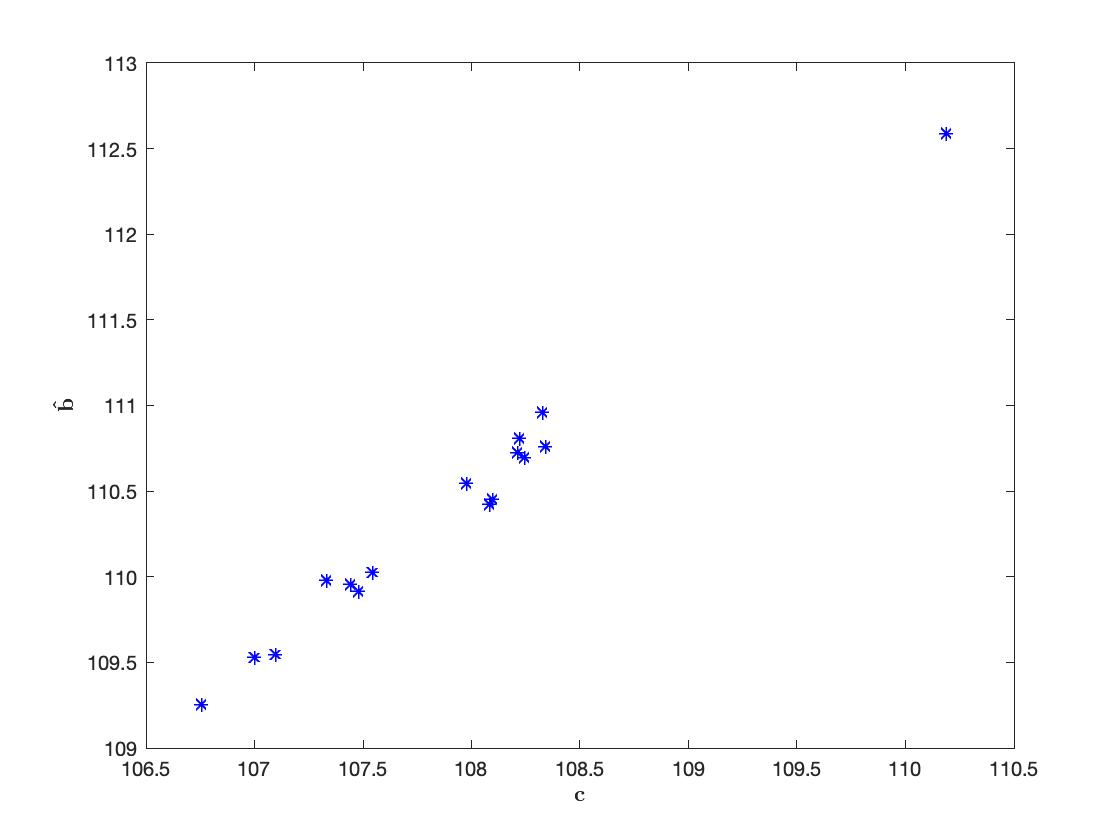
\includegraphics[width=1\linewidth]{simulated_bids.jpg}
        \caption{Simulated bids against simulated costs.}
        \label{fig:simulation}
    \end{minipage}%
    \begin{minipage}[h]{0.55\textwidth}
        \centering
        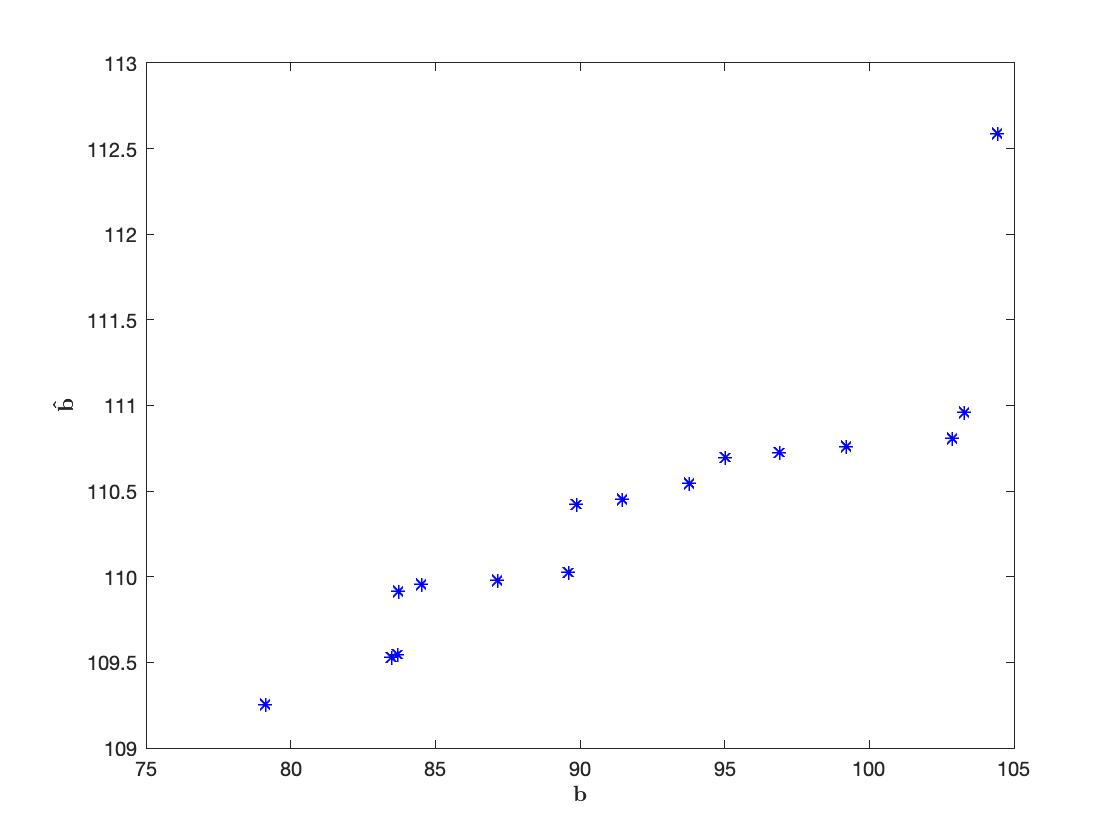
\includegraphics[width=1\linewidth]{actualVsimulated.jpg}
        \caption{Bids from test data (x-axis) plotted 
        against simulated bids (y-axis).}
        \label{fig:actualVsimulation}
    \end{minipage}
\end{figure}

Figure \ref{fig:simulation} plots simulated costs against simulated bids that are 
inferred from simulated costs using equation (\ref{eqn:BiddingFunction}). 
The simulated costs and bids center around 110\% 
and the range is small, with the max and min differing by less than 4\%. This 
is due to the estimated unimodal cost distribution 
concentrating in the range [80, 200], with a peak around 110\%. 
With the inversion method repeated 1000 times, it is natural that 
the costs and bids fall into the place where most bids and costs are 
concentrated. With the number of runs curtailed to 100 and 50, as shown in 
Figure \ref{fig:simulation_run_times}, the bids become more spread out and 
closer to the bid distribution. This shows that the number of runs is 
an important factor to determine to have a more accurate simulation 
but it is outside the scope of this paper. For simplicity, I will keep 
referencing the data generated with 1000 runs. 

\begin{figure}
\centering
    \begin{minipage}[h]{0.5\textwidth}
        \centering 
        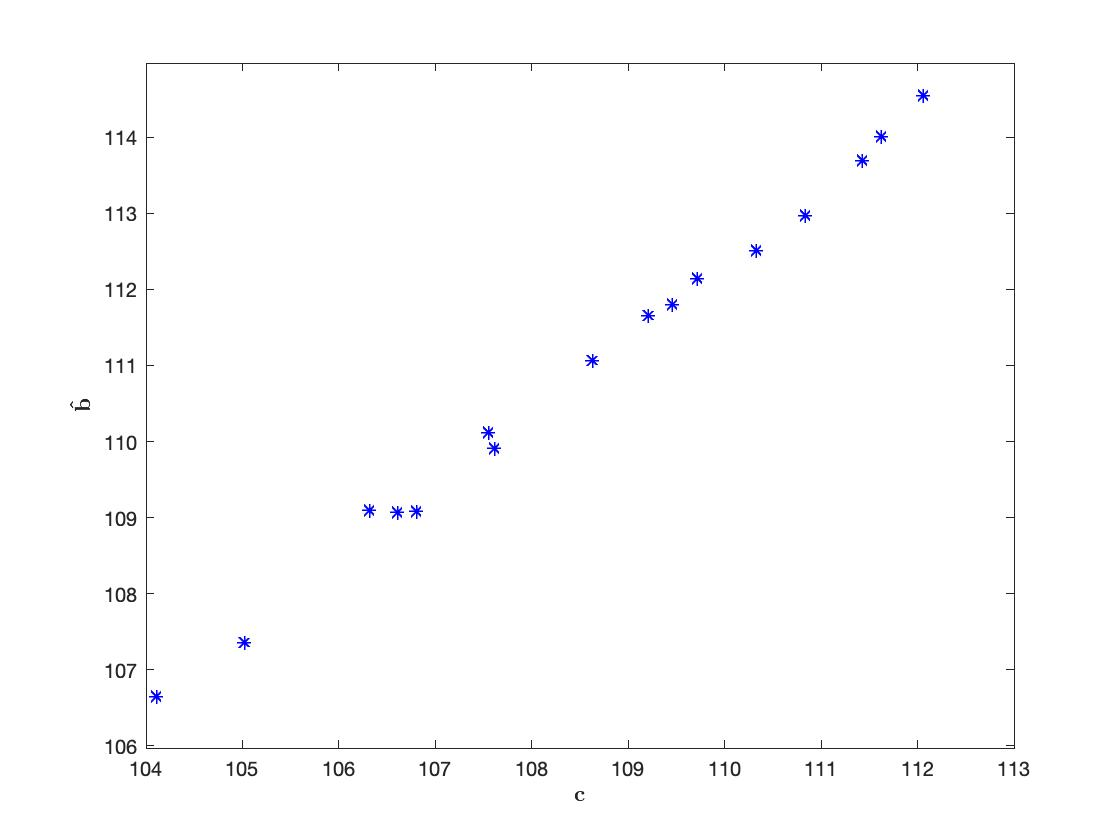
\includegraphics[width=\linewidth]{100run.jpg}
    \end{minipage}%
    \begin{minipage}[h]{0.5\textwidth}
        \centering
        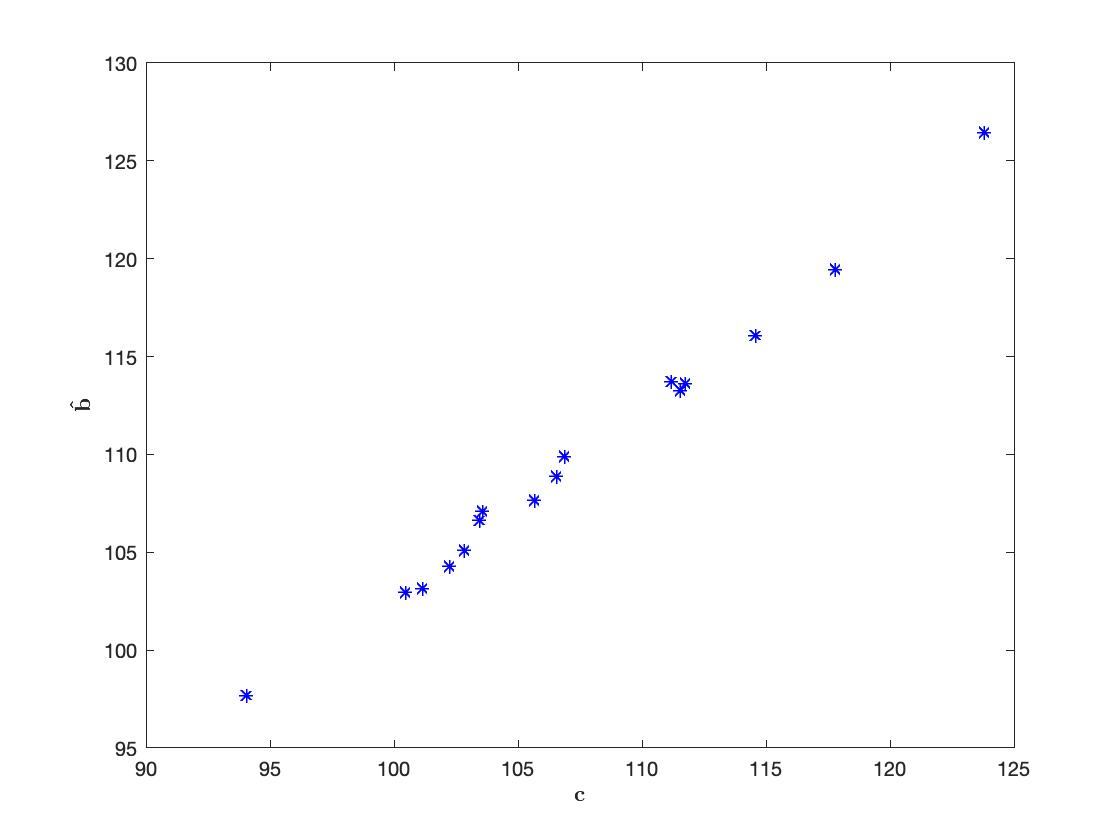
\includegraphics[width=\linewidth]{10run.jpg}
    \end{minipage}
\caption{Bid simulation run for 100 times (left) and 10 times(right)}
\label{fig:simulation_run_times}
\end{figure}

Figure \ref{fig:actualVsimulation} plots test data against simulated bids. 
A wide difference between simulation and test data is observed here. 
This difference, however, is not unexpected for two reasons: 
(1) the test data, which contains an auction with 16 bidders, does not conform 
to the bid distribution depicted in Figure \ref{fig:BidFrequency}, and 
(2) I am comparing most likely bids predicted by the estimated cost distribution 
to a particular auction. Therefore, the difference here does not suggest the 
inaccuracy of the estimated cost distribution or the equilibrium model. 
Instead, this exercise suggests that a larger test dataset is needed 
to deliver more informative results. 

\section{Conclusion}
This paper tries to propose a way to validate models used in structural analysis 
by cross-validation. The dataset is split into training data and test 
data.
First, this paper conducts structural estimation on a government 
procurement auction dataset about highway constructions and estimates the 
cost distribution on the training data using a two-step nonparametric procedure.
Second, using the 
estimated cost distribution, the paper then constructs simulated bids with the 
inversion method and compare the simulation to test data. 
But the wide difference between the simulation and test data does not suggest
that the first-price sealed-bid equilibrium model introduced in 
\citeauthor{RileySamuelson1981} \citeyear{RileySamuelson1981}
is not a suitable model to predict bidder's 
behavior in real-world auctions. Instead, to draw a firm conclusion requires 
more data. 

Moreover, in the second step of the cross-validation procedure, comparing bids 
directly to test theory's validity may not be a good idea, as suggested in 
\citeauthor{Harrison1989} \citeyear{Harrison1989}. \citeauthor{Harrison1989}
\citeyear{Harrison1989} instead proposes to "evaluate subject behavior in the 
expected payoff space", which can be incorporated into future work of the project.

The idea of cross-validation has been an old idea in the machine learning 
literature as a way to compare performance across models. I, therefore, consider 
it a natural idea to introduce it into structural analysis. Structural estimation 
relies on the model's correctness in modeling agent's behavior, but the verification 
of models is left to lab experiments, not empirical data which holds the final 
authority on models. Hopefully, this paper's experiment would shed light on 
possible directions that structural analysis can head to become more robust. 


\medskip

\bibliographystyle{apacite}
\bibliography{references}


\end{document}